\documentclass[]{article}
\usepackage{lmodern}
\usepackage{amssymb,amsmath}
\usepackage{ifxetex,ifluatex}
\usepackage{fixltx2e} % provides \textsubscript
\ifnum 0\ifxetex 1\fi\ifluatex 1\fi=0 % if pdftex
  \usepackage[T1]{fontenc}
  \usepackage[utf8]{inputenc}
\else % if luatex or xelatex
  \ifxetex
    \usepackage{mathspec}
  \else
    \usepackage{fontspec}
  \fi
  \defaultfontfeatures{Ligatures=TeX,Scale=MatchLowercase}
\fi
% use upquote if available, for straight quotes in verbatim environments
\IfFileExists{upquote.sty}{\usepackage{upquote}}{}
% use microtype if available
\IfFileExists{microtype.sty}{%
\usepackage{microtype}
\UseMicrotypeSet[protrusion]{basicmath} % disable protrusion for tt fonts
}{}
\usepackage[margin=1in]{geometry}
\usepackage{hyperref}
\hypersetup{unicode=true,
            pdfborder={0 0 0},
            breaklinks=true}
\urlstyle{same}  % don't use monospace font for urls
\usepackage{longtable,booktabs}
\usepackage{graphicx,grffile}
\makeatletter
\def\maxwidth{\ifdim\Gin@nat@width>\linewidth\linewidth\else\Gin@nat@width\fi}
\def\maxheight{\ifdim\Gin@nat@height>\textheight\textheight\else\Gin@nat@height\fi}
\makeatother
% Scale images if necessary, so that they will not overflow the page
% margins by default, and it is still possible to overwrite the defaults
% using explicit options in \includegraphics[width, height, ...]{}
\setkeys{Gin}{width=\maxwidth,height=\maxheight,keepaspectratio}
\IfFileExists{parskip.sty}{%
\usepackage{parskip}
}{% else
\setlength{\parindent}{0pt}
\setlength{\parskip}{6pt plus 2pt minus 1pt}
}
\setlength{\emergencystretch}{3em}  % prevent overfull lines
\providecommand{\tightlist}{%
  \setlength{\itemsep}{0pt}\setlength{\parskip}{0pt}}
\setcounter{secnumdepth}{0}
% Redefines (sub)paragraphs to behave more like sections
\ifx\paragraph\undefined\else
\let\oldparagraph\paragraph
\renewcommand{\paragraph}[1]{\oldparagraph{#1}\mbox{}}
\fi
\ifx\subparagraph\undefined\else
\let\oldsubparagraph\subparagraph
\renewcommand{\subparagraph}[1]{\oldsubparagraph{#1}\mbox{}}
\fi

%%% Use protect on footnotes to avoid problems with footnotes in titles
\let\rmarkdownfootnote\footnote%
\def\footnote{\protect\rmarkdownfootnote}

%%% Change title format to be more compact
\usepackage{titling}

% Create subtitle command for use in maketitle
\newcommand{\subtitle}[1]{
  \posttitle{
    \begin{center}\large#1\end{center}
    }
}

\setlength{\droptitle}{-2em}
  \title{}
  \pretitle{\vspace{\droptitle}}
  \posttitle{}
  \author{}
  \preauthor{}\postauthor{}
  \date{}
  \predate{}\postdate{}


\begin{document}

\subsection{\texorpdfstring{Example data formats for the sDIV project
\emph{sEcoEvo: Biodiversity Dynamics -- The Nexus Between Space \&
Time}}{Example data formats for the sDIV project sEcoEvo: Biodiversity Dynamics -- The Nexus Between Space \& Time}}\label{example-data-formats-for-the-sdiv-project-secoevo-biodiversity-dynamics-the-nexus-between-space-time}

Here we provide example data for all the different data types we are
interested in gathering for communities.

\begin{itemize}
\item
  Time calibrated trees (with branch lengths even if unresolved)

  \begin{quote}
  An example tree in Newick format is in the file
  \textbf{example.newick}. Please note that trees can include both
  sampled and unsampled lineages (the example tree includes 7 lineages
  that were not sampled in the local community). The structure of the
  tree looks like this:
  \end{quote}
\end{itemize}

\begin{center}
  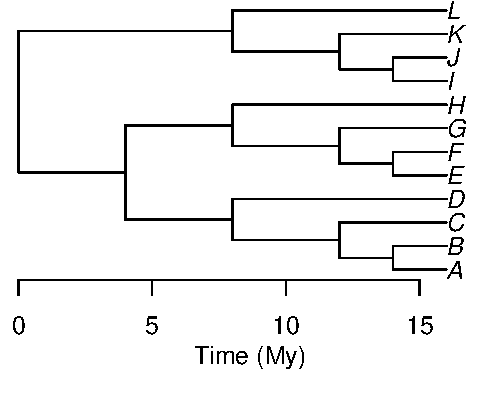
\includegraphics{example_tree.pdf}
\end{center}


\begin{itemize}
\item
  Abundances

  \begin{quote}
  We provide an example site-by-species file including 3 sites and the 5
  sampled species (B, D, E, F, \& K) in the file
  \textbf{example\_abundances.csv}. This is a simple CSV file with rows
  corresponding to sites, and columns corresponding to species, cells
  contain the abundance of each species at each site.
  \end{quote}
\end{itemize}

\begin{longtable}[]{@{}lrrrrr@{}}
& B & D & E & F & K\tabularnewline
site1 & 0 & 8 & 2 & 5 & 7\tabularnewline
site2 & 8 & 0 & 8 & 1 & 2\tabularnewline
site3 & 0 & 0 & 3 & 8 & 15\tabularnewline
\end{longtable}

\begin{itemize}
\item
  Per location per taxon sequence data (including identical sequences).

  \begin{quote}
  Example sequence data is shown in the \textbf{fastqs/} directory, with
  one fastq file per site, including all sequences for all individuals
  sequenced at that site. We will use these sequences to calculate
  nucleotide diversity per species per site.
  \end{quote}
\item
  Sample/species/site mapping file

  \begin{quote}
  Sequence data need to be matched to species and sites. We include an
  example file called \textbf{example\_pops.csv} which does this. This
  is CSV where each row contains 3 items, the sample id (which should
  match the sample name in the fastq files), the species ID (which
  should match the ID in the newick tree), and the sample site (which
  should match the site name in the abundances file).
  \end{quote}
\end{itemize}

\begin{longtable}[]{@{}lll@{}}
\toprule
sample\_ID & species & site\tabularnewline
\midrule
\endhead
B\_0\_1 & B & site1\tabularnewline
B\_1\_1 & B & site1\tabularnewline
B\_2\_1 & B & site1\tabularnewline
B\_3\_1 & B & site1\tabularnewline
B\_4\_1 & B & site1\tabularnewline
D\_0\_1 & D & site1\tabularnewline
\bottomrule
\end{longtable}

\begin{itemize}
\item
  Site metadata file

  \begin{quote}
  We need to know a few things about sites, most importantly their
  goegraphic locations, and hopefully also something about sampling
  methodology such as area, effort, sampling technique. The included
  example file \textbf{site\_metadata.csv} refers to arthropod pitfall
  trapping as an example.
  \end{quote}
\end{itemize}

\begin{longtable}[]{@{}lrrll@{}}
\toprule
site & lon & lat & method & duration\tabularnewline
\midrule
\endhead
site1 & -155.5134 & 19.23092 & pitfall & 5 days\tabularnewline
site2 & -155.5167 & 19.23250 & pitfall & 5 days\tabularnewline
site3 & -155.5155 & 19.23053 & pitfall & 5 days\tabularnewline
\bottomrule
\end{longtable}


\end{document}
